La figura muestra un sólido del primer octante limitado por el plano $x=0$, el cilindro parabólico $y=\sqrt{x}$, el plano $z=0$ y el plano inclinado $z=1-y$. Escriba $\iiint_E f(x,y,z)\,dV$ en los órdenes $dx\,dz\,dy$ y $dz\,dx\,dy$.

\begingroup
\shorthandoff{>}
\begin{center}
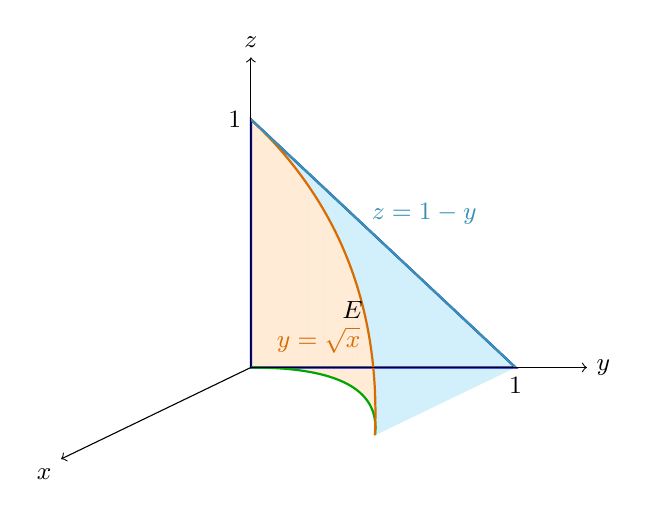
\begin{tikzpicture}[
    x={(-1.7cm,-.82cm)},y={(3.2cm,0cm)},z={(0cm,3cm)},
    scale=1.05,every node/.style={font=\small}]
    \fill[blue!11] (0,0,0) -- (0,1,0) -- (0,0,1) -- cycle;
    \fill[green!13] plot[domain=0:1,samples=35] ({\x*\x},{\x},0)
        -- (0,1,0) -- (0,0,0) -- cycle;
    \foreach \i in {0,...,11} {
        \pgfmathsetmacro{\ya}{\i/12}
        \pgfmathsetmacro{\yb}{(\i+1)/12}
        \fill[cyan!18]
            (0,\ya,{1-\ya}) -- ({\ya*\ya},\ya,{1-\ya}) --
            ({\yb*\yb},\yb,{1-\yb}) -- (0,\yb,{1-\yb}) -- cycle;
        \fill[orange!16]
            ({\ya*\ya},\ya,0) -- ({\yb*\yb},\yb,0) --
            ({\yb*\yb},\yb,{1-\yb}) -- ({\ya*\ya},\ya,{1-\ya}) -- cycle;
    }
    \draw[blue!75!black,thick] (0,0,0) -- (0,1,0) -- (0,0,1) -- cycle;
    \draw[green!65!black,thick]
        plot[domain=0:1,samples=45] ({\x*\x},{\x},0);
    \draw[orange!85!black,thick]
        plot[domain=0:1,samples=45] ({\x*\x},{\x},{1-\x});
    \draw[cyan!70!black,thick] (0,0,1) -- (0,1,0);
    \draw[->] (0,0,0) -- (1.35,0,0) node[below left] {$x$};
    \draw[->] (0,0,0) -- (0,1.27,0) node[right] {$y$};
    \draw[->] (0,0,0) -- (0,0,1.25) node[above] {$z$};
    \node[left] at (0,0,1) {$1$};
    \node[below] at (0,1,0) {$1$};
    \node[orange!85!black,left] at (.62,.78,.28) {$y=\sqrt{x}$};
    \node[cyan!70!black,right] at (0,.42,.62) {$z=1-y$};
    \node at (.18,.48,.28) {$E$};
\end{tikzpicture}
\end{center}
\endgroup
